\documentclass[10pt,letterpaper,final,twoside,notitlepage]{article}
\usepackage[margin=.5in]{geometry}
\usepackage[utf8]{inputenc}
\usepackage[english]{babel}
\usepackage{amsmath}
\usepackage{amsfonts}
\usepackage{amssymb}
\usepackage{amsthm} % Gives us plain, definition, and remark to use in \theoremstyle{style}
\usepackage{graphicx}

\usepackage{subfigure} % Float environment to place multiple figures in one figure environment
\usepackage{nameref} % \nameref{label} lets you reference things by name
\usepackage{hyperref} % Hyperlinks between references
\usepackage{enumitem} % Provides [noitemsep, nolistsep] for more compact lists
\usepackage{chngcntr} % Allows us to tamper with the counter a little more

\graphicspath{./Drawings/Phys_224/} % Uncomment this to use pictures in this document

\numberwithin{equation}{section} % Uncomment this to number equations with section numbers too

\theoremstyle{definition}
\newtheorem{definition}{Defn}

\theoremstyle{remark}
\newtheorem{note}{Note}

\author{Karl Hallsby}
\title{Phys 224 Reference Sheet}

\begin{document}
\section{General Stuff} \label{sec:General}
	\begin{itemize}[noitemsep]
		\item Density - $\rho = \frac{\Delta m}{\Delta V}$
			\begin{itemize}
				\item Uniform Density - $\rho = \frac{m}{V}$
			\end{itemize}
		
		\item Pressure - $p = \frac{\Delta F}{\Delta A}$
			\begin{itemize}
				\item Uniform Force on Flat Area - $\rho = \frac{F}{A}$
				\item Conversions - $1 atm = 1.01 \times 10^5 Pa = 760 torr = 14.7 lb/in^2$
			\end{itemize}
		\item Trig Relations are in \nameref{subsubsec:Trig Formulas}, Section~\ref{subsubsec:Trig Formulas}.
	\end{itemize}

\section{Fluids} \label{sec:Fluids}
We must satisfy several parameters to make life easier, and to use most of these formulae.
	\begin{enumerate}[noitemsep]
		\item Incompressible - Density of the fluid is constant
		\item Non-turbulent Flow - Think of fluids swirling around an object
		\item Isostatic Pressure - Pressure inside the fluid is the same in all directions
	\end{enumerate}

	\begin{itemize}[noitemsep]
		\item Pressure at Some Depth - $p_{2} = p_{1} + \rho g \left( y_{1}-y_{2} \right)$
			\begin{itemize}
				\item Pressure at Depth $h \rightarrow p = p_{0} + \rho gh$
			\end{itemize}
		\item Pascal's Principle - 2 Parts
			\begin{enumerate}[noitemsep]
				\item $\vec{F_{o}} = \vec{F}_{i}\ \frac{A_{o}}{A_{i}}$
				\item $d_{o} = d_{i} \frac{A_{i}}{A_{o}}$
			\end{enumerate}
		\begin{itemize}[noitemsep, nolistsep]
			\item When 2 pressures should be equal, their forces are inversely proportional
			\item Set each pressure equal to each other, then solve for the missing variable.
		\end{itemize}
		\item Archimedes' Principle - $\vec{F}_{Up} = \vec{F}_{Down}$
			\begin{itemize}[noitemsep]
				\item Usually breaks down to $\vec{F}_{Bouyant} = \vec{F}_{g, Object}$
				\item $\vec{F}_{Bouyant} = m_{Object}g$
				\item $\vec{F}_{Bouyant} = \rho_{Object}V_{Object}g$
			\end{itemize}
		\item Continuity of Fluids
		\begin{itemize}[noitemsep]
			\item $A_{1}v_{1} = A_{2}v_{2}$
		\end{itemize}
		\item Bernoulli's Equation - $p_{1} + \frac{1}{2} \rho v_{1}^{2} + \rho gy_{1} = p_{2} + 	\frac{1}{2} \rho v_{2}^{2} + \rho gy_{2}$
			\begin{itemize}[noitemsep]
				\item Fluids at Rest - $p_{2} = p_{1} + \rho g \left( y_{1}-y_{2} \right)$
				\item Fluids not Changing Height - $p_{1} + \frac{1}{2} \rho v_{1}^{2} = p_{2} + 	\frac{1}{2} \rho v_{2}^{2}$
			\end{itemize}
	\end{itemize}

\section{Waves} \label{sec:Waves}
{\Large Usually of form $y = y_{m} \sin \left( kx \pm \omega t \right)$}
There are two types of waves:
	\begin{enumerate}[noitemsep, nolistsep]
		\item Transverse Waves - Waves where displacement from equilibrium is orthogonal to direction of propagation
		\begin{itemize}[noitemsep, nolistsep] % Examples of Transverse Waves
			\item String Waves
			\item Electromagnetic Waves
		\end{itemize}
		\item Longitudinal Waves - Waves where displacement from equilibrium is parallel to direction of propagation
		\begin{itemize}[noitemsep, nolistsep] % Examples of Longitudinal Waves
			\item Pressure Waves
			\item Sound Waves (Which are a type of pressure wave)
		\end{itemize}
	\end{enumerate}

	\begin{itemize}[noitemsep]
		\item $y_{m}$ - Amplitude, $m$
		\item $k$ - Angular Wave Number, $rad/m$
			\begin{itemize}[noitemsep, nolistsep]
				\item $k = \frac{2 \pi}{\lambda}$
				\item $\lambda$ is wavelength, $m$
			\end{itemize}
		\item $\omega$ - Angular Frequency, $rad/s$
			\begin{itemize}[noitemsep, nolistsep]
				\item $\omega = 2 \pi f$
				\item $f$ is frequency, $Hz$
				\item Sign of this goes the opposite the direction the wave is going
					\begin{enumerate}[noitemsep]
						\item Wave going in positive direction $\left( + \right)$, then the sign should be negative $\left( - \right)$
						\item Wave going in negative direction $\left( - \right)$, then the sign should be positive $\left( + \right)$
					\end{enumerate}
			\end{itemize}
		\item $v = \lambda f$, Wave Velocity, $m/s$
			\begin{itemize}[noitemsep]
				\item $v = \frac{\omega}{2 \pi} * \frac{2 \pi}{k} = \frac{\omega}{k}$
				\item This can be proven with the angular portion of any wave (inside the parentheses of trig function)
				\begin{align*} % Prove why k = \lambda / 2 \pi
					kx-\omega t &= \text{Constant} \\
					\frac{d}{dt} \left[ kx-\omega t \right] &= \frac{d}{dt} \left[ \text{Constant} \right] \\
					k \frac{dx}{dt} - \omega \frac{dt}{dt} &= 0 \\
					kv - \omega &= 0 \\
					kv &= \omega \\
					v &= \frac{\omega}{k} \\
				\end{align*}
				Since $\omega = 2 \pi f$ , then $k = \frac{\lambda}{2 \pi}$ 
			\end{itemize}
	\end{itemize}

	\subsection*{Wave Interference} \label{subsec:Wave Interference}
	Waves are nice, and they just sum when they interfere. Let: 
	\begin{align}
		y_{1} \left( x, t \right) &= y \sin \left( kx - \omega t \right) \\
		y_{2} \left( x, t \right) &= y \sin \left( kx + \omega t + \varphi \right) \\
		Y \left( x, t \right) &= y\left[ \sin \left( kx - \omega t \right) + \sin \left( kx + \omega t + \varphi \right) \right] \label{eq:Sum of 2 Waves}
	\end{align}
	You can usually use Equation~\ref{eq:Sin plus Sin with diff Angles} to simplify Equation~\ref{eq:Sum of 2 Waves}.

		\subsubsection*{Constructive/Destructive Interference} \label{subsubsec:Constructive/Destructive Interference}
		\begin{align*}		
			\phi &= 2 \pi \frac{Path Length Diff}{\lambda} = 2 \pi \frac{\Delta \text{PLD}}{\lambda} \\
			n &= \frac{\phi}{2\pi} = 4 \frac{Path Length Diff}{\lambda}\\
		\end{align*}
		\begin{itemize}[noitemsep]
			\item $Path Length Diff$ - Is the Difference in path lengths that the waves must travel
			\item $phi$ - Angular Location of points of Complete Constructive/Destructive Interference
			\item $n$ - Number of locations where there is Complete Constructive/Destructive Interference
		\end{itemize}

	\subsection*{Standing Waves} \label{subsec:Standing Waves}
	This is actually the superposition of 2 waves, traveling in opposite directions, on a medium that is fixed at both ends, i.e. a taut string held by a wall.
		\subsubsection*{Location of Nodes and Antinodes} \label{subsubsec:Node/Antinode Location}
		\begin{itemize}[noitemsep]
			\item Nodes - $x = n \frac{\lambda}{2}$ for $n = 0, 1, 2, \ldots$
			\begin{itemize}[noitemsep, nolistsep]
				\item Always at closed ends of tubes
			\end{itemize}
			\item Antinodes - $x = \left( n + \frac{1}{2} \right) \frac{\lambda}{2}$ for $n = 0, 1, 2, \ldots$
			\begin{itemize}[noitemsep, nolistsep]
				\item Always at open ends of tubes
			\end{itemize}
		\end{itemize}

		\subsubsection*{Resonant Frequencies/Harmonics} \label{subsubsec:Resonant Frequencies/Harmonics}
		These can also be called harmonics. There is a resonant frequency for every number of nodes/antinodes on tthe standing wave. \newline
		$f = \frac{v}{\lambda} = n \frac{v}{2L}$
		\begin{itemize}[noitemsep]
			\item $L$ is the length of the medium (The String).
			\item $\lambda$ is the wavelength of the wave formed.
		\end{itemize}
		This can be extended to find the base resonant frequency, if you know how many node levels are between the two resonant frequencies given, i.e. they say that the \textbf{NEXT} frequency, means $n+1$. \newline
		$f_{n+m}-f_{n} = \left( n+m \right) \frac{v}{2L} - n \frac{v}{2L} = m \frac{v}{2L}$
		
	\subsection*{Reflecting Sound} \label{subsec:Reflecting Sound}
		\begin{itemize}[noitemsep]
			\item $D = \left( n + 1 \right)d = vt$
			\begin{itemize}[noitemsep,nolistsep]
				\item $n$ is the number of reflections that occurred
				\item $n+1$ is used when we want the distance the wave covers
			\end{itemize}
		\end{itemize}
	
	\subsection*{Sound in Different Mediums} \label{subsec:Sound in Different Mediums}
	Frequency is a property of a wave, and \textbf{CANNOT BE ALTERED.} This means that:
	\begin{align*}
		v &= \lambda f \\
		v_{Sound, Material 1} &= \lambda_{Material 1}f_{Unique, Material 1} \\
		v_{Sound, Material 2} &= \lambda_{Material 2}f_{Unique, Material 2} \\
		f_{Unique, Material 1} &= f_{Unique, Material 2} \\
		\frac{v_{Sound, Material 1}}{\lambda_{Material 1}} &= \frac{v_{Sound, Material 2}}{\lambda_{Material 2}} \\
	\end{align*}
	
	\subsection*{Doppler Effect} \label{subsec:Doppler Effect}
	{\Large $f' = f \frac{v \pm v_{D}}{v \pm v_{S}}$}
	\begin{itemize}[noitemsep]
		\item Moving \textit{\textbf{TOWARDS}} each other: Frequency Increase
		\item Moving \textit{\textbf{AWAY}} from each other: Frequency Decrease
		\item $f$ - Initial Frequency, $Hz$
		\item $v$ - Sound Speed, $m/s$
		\item $v_{D}$ - Detector Speed, $m/s$
		\item $v_{S}$ - Source Speed, $m/s$
		\item \textbf{For Numerator}:
			\begin{itemize}[noitemsep,nolistsep]
				\item If detector is moving towards the source, $+$
				\item If detector is moving away from the source, $-$
			\end{itemize}
		\item \textbf{For Denominator}:
			\begin{itemize}[noitemsep,nolistsep]
				\item If source is moving away from detector, $+$
				\item If source is moving towards the detector, $-$
			\end{itemize}
		\end{itemize}

\section{Thermodynamics} \label{sec:Thermo}
	\begin{definition}[Thermodynamics] \label{def:Thermo}
		\emph{Thermodynamics} is the study of energy transfer between two macroscopic bodies driven by temperature differences.
	\end{definition}
	\begin{definition}[Temperature] \label{def:Temperature}
		\emph{Temperature} is a direct measurement of internal energy of a system
	\end{definition}

	\subsection*{Laws of Thermodynamics} \label{subsec:Thermo Laws}
		\begin{definition}[0th Law of Thermodynamics] \label{def:0th Law of Thermo}
			If 2 bodies, A and B are in thermal equilibrium with a third body ``T'', then they are in thermal equilibrium with each other.
		\end{definition}
		\begin{definition}[1st Law of Thermodynamics] \label{def:1st Law of Thermo}
			\begin{equation} \label{eq:1st Law of Thermo}
				dE_{Internal} = dQ - dT \text{, } dQ \text{ and } dT \text{ are inexact (path-dependent) differentials.}
			\end{equation}
			\textbf{Special Cases for the 1st Law of Thermodynamics}:
			\begin{enumerate}[noitemsep, nolistsep]
				\item Adiabatic Processes - $dE_{Int} = -dW$
				\begin{itemize}[noitemsep, nolistsep]
					\item No heat exchange
					\item Insulating
					\item Something happens too quickly for system to keep up
				\end{itemize}
				\item Isothermal Processes - $dT = 0 \rightarrow dE_{Int} = 0 \rightarrow dQ = dW$
				\item Isobaric Processes - $dW = pdV$, $p$(pressure) is constant
				\item Cyclical Processes - $dE_{Int} = 0 \rightarrow dQ = dW$
				\begin{itemize}[noitemsep, nolistsep]
					\item You end a cycle with the same internal energy when the cycle started
				\end{itemize}
			\end{enumerate}
		\end{definition}
		\begin{definition}[2nd Law of Thermodynamics] \label{def:2nd Law of Thermo}
			If a \emph{cyclical process occurs in a CLOSED system}, the entropy of the system increases for irreversible processes and remains constant for reversible processes. \textbf{IT NEVER DECREASES!!}
			\begin{align} \label{eq:2nd Law of Thermo}
				\Delta S &\geq 0 \\
				\Delta S &= \int_{a}^{b} \frac{dQ \left( T \right)}{T} 
			\end{align}
			\textbf{$\mathbf{\Delta S}$ is a state-function, meaning it is path-independent.}
		\end{definition}
	
	\subsection*{Heat and Work} \label{subsec:Heat/Work}
		\begin{itemize}[noitemsep, nolistsep]
			\item $dW = \vec{F} \dot \vec{ds}$
			\item $\vec{F} = p \left( V, T \right) dV$
			\item $W = \int p \left( V, T \right) dV$
			\item $W = \frac{dQ}{dt}$
			\item $W = \frac{\Delta Q}{\Delta t}$
		\end{itemize}
	\emph{\textbf{Work done by thermal energy is path independent.}}

	\subsection*{Thermal Expansion} \label{subsec:Thermal Expansion}
	Occurs because the ``springs'' between each of the atoms in a lattice have energy applied by Heat (Temperature Change).
		\begin{itemize}
			\item $\frac{\Delta L}{L_{0}} = \alpha \Delta T$ (One-Dimensional Expansion)
			\item $\frac{dL}{L_{0}} = \alpha dT$ (One-Dimensional Expansion)
			\begin{itemize}[noitemsep, nolistsep]
				\item $\alpha$ is a material-specific constant
			\end{itemize}
		\end{itemize}
	
	\subsection*{Specific Heat/Heat Capacity} \label{subsec:Specific Heat/Heat Capacity}
		\begin{itemize}
			\item $C = \frac{dQ}{dT} \leftarrow$ Specific Heat
			\item $c = \frac{dQ}{mdT} \leftarrow$ Mass Specific Heat
		\end{itemize}
	
	\subsection*{Heat of Phase Transitions} \label{subec:Heat Phase Transitions}
	This is a constant unique to the material and the phase transition it is going through.
	\begin{itemize}[nolistsep]
		\item $Q = Lm$
		\item $Q = \int_{m_{i}}^{m_{f}} L_{f} dm$
		\begin{itemize}[noitemsep, nolistsep]
			\item $l_{Fusion} = $ Heat required to turn things from \textbf{SOLID TO LIQUID}
			\item $l_{Vapor} = $ Heat required to turn things from \textbf{LIQUID TO GAS}
		\end{itemize}
	\end{itemize}

	\subsection*{Conduction Heat Transfer} \label{subsec:Conduction Heat Transfer}
	\begin{equation} \label{eq:Conduction Heat Transfer}
		P_{Conduction} = \frac{\left( T_{H} - T_{C} \right)}{L} Ak
	\end{equation}
		\begin{itemize}[noitemsep, nolistsep]
			\item $L$ = Length
			\item $A$ = Cross-Sectional Area
			\item $k$ = Material's Thermal Conductivity
		\end{itemize}
	For multiple materials between 2 thermal reservoirs:
	\begin{itemize}[noitemsep, nolistsep]
		\item $P_{1} = P_{2} = \ldots = P_{n}$
		\item Heat will only flow as fast as the slowest thermal conductor
	\end{itemize}

\section{Kinetic Theory of Ideal Gases} \label{sec:Kinetic Theory of Ideal Gases}
	\begin{definition}[Ideal Gas] \label{def:Ideal Gas}
		An \emph{ideal gas} is a gas that obeys the ideal gas law.
		\begin{equation} \label{eq:Ideal Gas Law}
			pV = nRT \text{, } R \approxeq 8.31 J/mol K
		\end{equation}
	\end{definition}

	\subsection*{Work Done by Ideal Gases} \label{subsec:Work Done By Ideal Gas}
		\subsubsection*{Isothermally} \label{subsubsec:Work Done Isothermally}
			\begin{equation}
				\begin{aligned}
					W &= \int \vec{F} \vec{ds} \\
					W &= \int_{V_{1}}^{V_{2}} p \left( V,T \right) dV \\
					W &= \int_{V_{1}}^{V_{2}} \frac{nRT}{V} dV \\
					W &= nRT \int_{V_{1}}^{V_{2}} \frac{1}{V} dV \\
					W &= nRT \ln \left( \frac{V_{2}}{V_{1}} \right) \\
				\end{aligned}
			\end{equation}
		\subsubsection*{Constant Pressure} \label{subsubsec:Work Done Under Constant Pressure}
			\begin{equation}
				W = p \left(V_{final}-V_{init} \right)
			\end{equation}
			
	\subsection*{Translational Kinetic Energy} \label{subsec:Translational Kinetic Energy}
		\begin{definition}[Degrees of Freedom] \label{def:Degrees of Freedom}
			\emph{Degrees of freedom} represent the number of variables that are needed to describe a system. Represented with $d$, occasionally.
			\begin{note}
				In an ideal gas, these are a means to store energy.
			\end{note}
		\end{definition}
	
		\begin{table}[h!]
			\centering
			\begin{tabular}{c|c|c|c}
				(Blank) & Translational & Rotational & Total \\ \hline
				Monatomic & 3 & 0 & 3 \\ \hline
				Diatomic & 3 & 2 & 5 \\ \hline
				Polyatomic & 3 & 3 & 6 \\
			\end{tabular}
			\caption{Degrees of Freedom Table for Gases}
			\label{tab:Degrees of Freedom}
		\end{table}
		\begin{itemize}[noitemsep, nolistsep]
			\item An ideal gas has \emph{\textbf{ONLY}} kinetic energy
			\item Completely elastic collisions
		\end{itemize}
		
		\begin{equation} \label{eq:Internal Energy of Ideal Gas}
			E_{int} = \frac{DoF}{2} nRT \text{, where } DoF=\text{Degrees of Freedom}
		\end{equation}
		
	\subsection*{Molar Specific Heats of Ideal Gases} \label{subsec:Molar Specific Heats of Ideal Gases}
		\subsubsection*{Molar Specific Heat @ Constant Volume} \label{subsubsec:Molar Specific Heat @ Constant Volume}
			\begin{equation} \label{eq:Molar Specific Heat @ Constant Volume}
				\begin{aligned}
					C_{V} &= \frac{\Delta E}{n \Delta T} \\
					C_{V} &= \frac{dE}{dT} \\
					C_{V} &= \left( \frac{DoF}{2} \right) R \\
				\end{aligned}
			\end{equation}
		\subsubsection*{Molar Specific Heat @ Constant Pressure} \label{Molar Specific Heat @ Constant Pressure}
			\begin{equation} \label{eq:Molar Specific Heat @ Constant Pressure}
				C_{P} = C_{V} + R
			\end{equation}
		
		
\section{Entropy} \label{sec:Entropy}
There is a heavy relationship between this and the \nameref{def:2nd Law of Thermo}.
	\begin{definition}[Entropy] \label{def:Entropy}
		\emph{Entropy} is a measure of the number of available states.
		\begin{equation} \label{eq:Entropy}
			S = k_{B} \ln \left( \Omega \right)
		\end{equation}
		\textbf{Entropy is NOT disorder.}
	\end{definition}

\section{Light} \label{sec:Light}
	\begin{definition}[Photon]
		A \emph{photon} is a wave propagating through an electric field.
	\end{definition}
The various $\theta$ used in Equations~\eqref{eq:Reflected Light},~\eqref{eq:Refracted Light} are measured from the surface normal.

\emph{Chromatic Dispersion} is the breaking up of polychromatic light by spectra.
Think of Pink Floyd's \textit{Dark Side of the Moon} album cover.
This happens because shorter wavelength, higher frequency light has a slightly higher index of refraction.
%	\begin{figure}[h!]
%		\centering
%		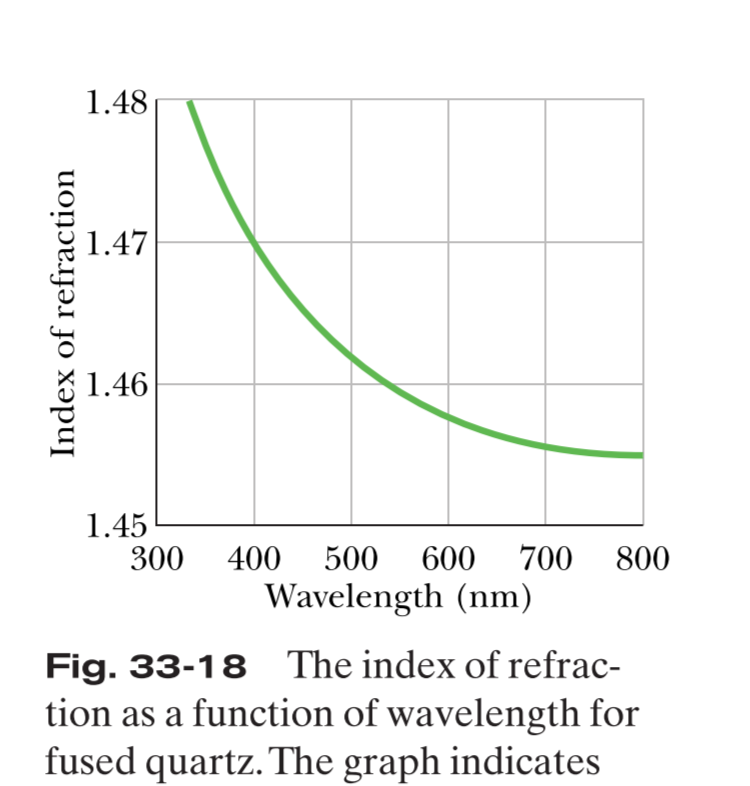
\includegraphics[scale=0.5]{Polychromatic_Light_Indices_Refraction.png}
%		\caption{Indices of Refraction for Polychromatic Light}
%		\label{fig:Indices of Refraction for Polychromatic Light}
%	\end{figure}

	\subsection*{Reflection} \label{subsec:Reflection}
		\begin{equation} \label{eq:Reflected Light}
			\theta_{reflected} = \theta_{incident}
		\end{equation}
		
	\subsection*{Refraction} \label{subsec:Refraction}
		\begin{definition}[Snell's Law] \label{def:Snell's Law}
			\begin{equation} \label{eq:Refracted Light} 
				n_{refract} \sin \left( \theta_{refract} \right) = n_{incident} \sin \left( \theta_{incident} \right)
			\end{equation}
		\end{definition}
		\begin{definition}[Index of Refraction] \label{def:Index of Refraction}
			\begin{equation} \label{eq:Index of Refraction}
				\begin{aligned}
					n_{i} &= \frac{c}{v_{i}} \\
					\lambda &= \frac{\lambda_{0}}{n} \\
				\end{aligned}
			\end{equation}
		\end{definition}
	
	\subsection*{Total Internal Reflection} \label{subsec:Total Internal Reflection}
		Total Internal Reflection occurs when the \emph{refracted light's angle is $\frac{\pi}{2}$}.
		\begin{equation} \label{eq:Total Internal Reflection}
			n_{refract} \sin \left( \theta_{refract} \right) = n_{incident} \sin \left( \theta_{incident} \right) \text{, where } \theta_{refract} = \frac{\pi}{2}
		\end{equation}
		
	\subsection*{Interference} \label{subsec:Light Interference}
		\begin{definition}[Huygen's Principle] \label{def:Huygen's Principle}
			Any point on a plane wavefront can be treated as a source of outgoing spherical waves.
			\begin{note}
				This is a mathematical construct/model.
			\end{note}
		\end{definition}

\section{Quantum Mechanics} \label{sec:Quantum Mech}

\appendix
\section{Reference Material} \label{sec:Reference Material}

\subsection{Physical Constants} \label{app:Physical Constants}
	\begin{table}[h!]
		\centering
		\begin{tabular}{|c|c|c|}
			\hline
			\textbf{Constant Name} & \textbf{Variable Letter} & \textbf{Value} \\ \hline
			Boltzmann Constant & $R$ & $8.314 \si{\joule / \mole~\kelvin}$ \\ \hline
			Universal Gravitational & $G$ & $6.67408 \times 10^{-11} \si{\meter^{3}~\kilogram^{-1}~\second^{-2}}$ \\ \hline
			Planck's Constant & $h$ & $6.62607004 \times 10^{-34} \si{\meter \kilogram / \second}$ \\ \hline
			Speed of Light & $c$ & $299792458 \si{\meter / \second}$ \\ \hline
			Mass of Earth & $m_{Earth}$ & $5.972 \times 10^{24} \si{\kilogram}$ \\ \hline
			Diameter of Earth & $d_{Earth}$ & $12742 \si{\kilo\meter}$ \\ \hline
		\end{tabular}
	\end{table}
\subsection{Trigonometry} \label{app:Trig}
	\subsubsection{Trigonometric Formulas} \label{subsubsec:Trig Formulas}
		\begin{equation} \label{eq:Sin plus Sin with diff Angles}
			\sin \left( \alpha \right) + \sin \left( \beta \right) = 2 \sin \left( \frac{\alpha + \beta}{2} \right) \cos\left( \frac{\alpha - \beta}{2} \right)  
		\end{equation}
		\begin{equation} \label{eq:Cosine-Sine Product}
			\cos \left( \theta \right) \sin \left( \theta \right) = \frac{1}{2} \sin \left( 2 \theta \right)
		\end{equation}
	
	\subsubsection{Euler Equivalents of Trigonometric Functions} \label{subsubsec:Euler Equivalents}
		\begin{equation} \label{eq:Euler Sin}
			\sin \left( x \right) = \frac{e^{\imath x} + e^{-\imath x}}{2}
		\end{equation}
		\begin{equation} \label{eq:Euler Cos}
			\cos \left( x \right) = \frac{e^{\imath x} - e^{-\imath x}}{2 \imath}
		\end{equation}
		\begin{equation} \label{eq:Euler Sinh}
			\sinh \left( x \right) = \frac{e^{x} - e^{-x}}{2}
		\end{equation}
		\begin{equation} \label{eq:Euler Cosh}
			\cosh \left( x \right) = \frac{e^{x} + e^{-x}}{2}
		\end{equation}

\end{document}